\chapter{Background}\label{ch:1}

\section{Visual sensory neuroscience}
In this section, we provide an introduction to visual neuroscience necessary for understanding the biological plausibility of our models. For a more comprehensive and in-depth introduction to neuroscience of vision please refer to \textit{Neuroscience: Exploring the Brain} (\cite{bear_neuroscience:_2007}) or the excellent summary provided as part of \cite{Carandini10577} review.

\subsection{Early visual system}\label{ch:1.1.1}
In this thesis we restrict our focus to the first 3 early stages of visual processing, corresponding to three neural structures: the retina, lateral geniculate body (LGN) and primary visual cortex (V1).

The journey of a visual stimuli starts on the retina at the back of an eye, where photosensitive cells - rods and cones measure the intensity of the light reflected by objects in our field of vision and projected at the back of our eye by cornea. While the particularities of rods and cones are interesting, especially when it comes to color processing, for the purpose of this introduction we will treat them as simple detectors that output electrical signal proportional to the sensed luminance, resulting in what could be abstracted as a matrix of luminescence levels - a raster image. 

The first processing step happens directly in the eye through retinal ganglion cells. Again, these cells are more complicated than presented here, but on a high level they detect local features such as contrast, directional movement of small stimuli, etc. The two main types are ON and OFF cells, both having a circular receptive field. Receptive field is the portion of sensory space that elicits neural responses when stimulated. In case of vision that means the section of the visual field a particular neuron responds to. ON cells fire when a high luminance hits the the center of its receptive fields and the disk at the edge is, proportionally, less excited. OFF cells function in the exact opposite way. For illustration, refer to Fig. \ref{fig:1.1}.

\begin{figure}
    \centering
    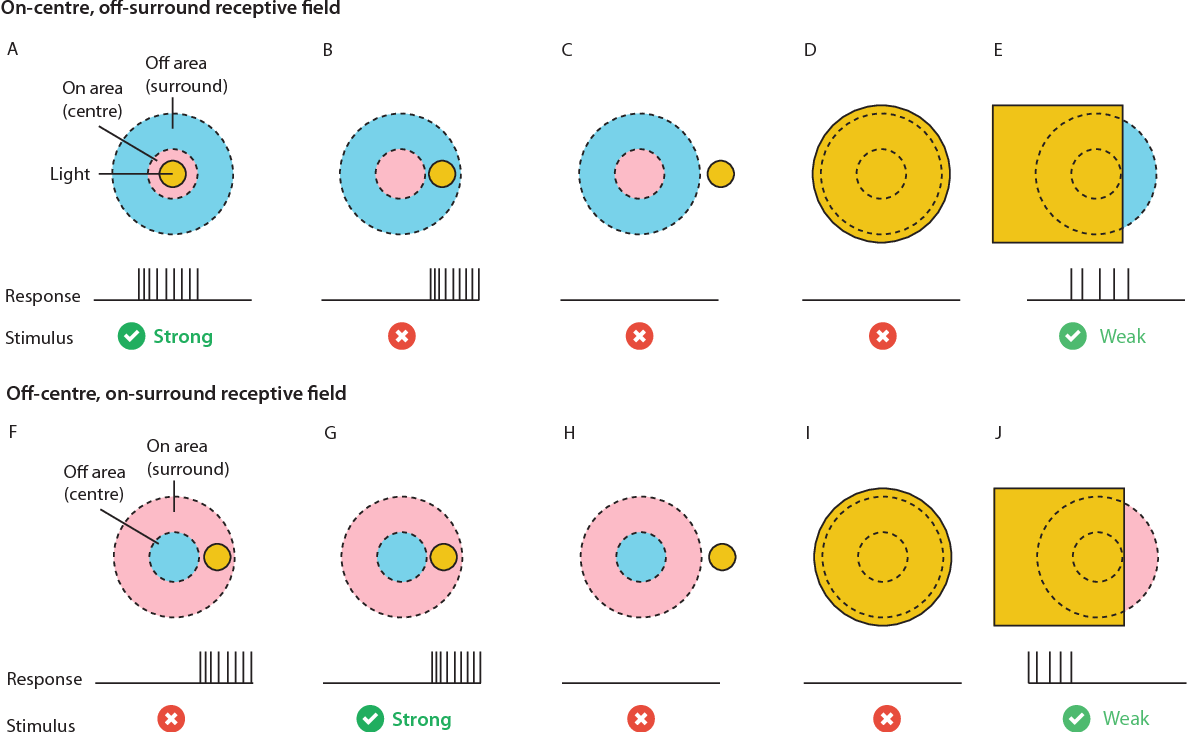
\includegraphics[width=1\textwidth]{../figures/01_33-Figure2.8-1}
    \caption[Receptive fields of retinal ganglion and LGN cells]{Receptive fields of retinal ganglion and LGN cells. Adapted from \cite{thesis_2015}.}
    \label{fig:1.1}
\end{figure}

From the eye most of the signal travels to LGN\footnote{Describing the visual pathway as a strictly feed-forward network is a great simplification.}, which serves as an active bridge to the visual cortex at the back side of the brain. Much like later V1, LGN is composed of 6 layers. The processing that happens here could be summarized as very similar to the retinal ganglion cells, only with bigger receptive fields. It is important to note that LGN does not get input only or even mainly from retina. It also receives substantial feedback from the primary visual cortex, and has synapses from parts of the thalamus and the brain stem. For example, the brain stem connection is believed to be responsible for perceived visual impacts of alertness changes, such as a flash of light when one is startled in a dark room. However, the exact role of these extra-retina sources in LGN function remains largely not understood. This means that the activity of both LGN, and all downstream stages of processing, such as V1, is modulated not only by the visual stimuli but also other neural activity inducing factors, for example emotions, locomotion, or other sensory inputs. Any models predicting the activity of LGN, V1, or higher stages of visual processing that are based solely on visual stimuli cannot, therefore, explain the entirety of recorded data. Nevertheless, under restricted experimental conditions, a wide range of studies have shown that the response of LGN cells can be very well approximated by a linear filter composed of difference-of-Gaussians. 

At last, the signal reaches the primary visual cortex. It is divided into 6 layers. Within V1, we recognize two main functional cell types - the so-called simple and complex cells. Simple cells, as their name suggests, can be represented as mostly linear combinations of ON and OFF cells. This means that within their receptive fields, they have well defined excitatory and inhibitory regions. In essence, they elicit response when stimulus, in this case light, hits the excitatory regions substantially more than the inhibitory regions. Their receptive field tends to be axis aligned, making them sensitive to oriented edges and gratings. They are also commonly described as Gabor-like filters (see Fig. \ref{fig:1.2}). 

\begin{figure}[ht]
    \centering
    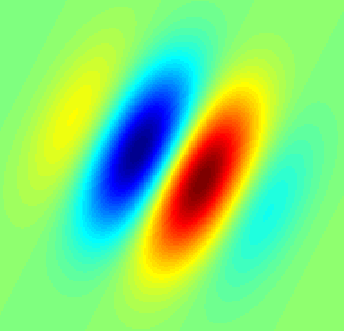
\includegraphics[width=0.3\textwidth]{../figures/01_Gabor_filter}
    \caption[Gabor filter-type receptive field typical for a simple cell]{Gabor filter-type receptive field typical for a simple cell. Blue regions indicate inhibition, red excitation. Figure was adopted from \cite{pict_gabor_filter}.}
    \label{fig:1.2}
\end{figure}

The nature of complex cells is not yet entirely settled, but it is understood that the relationship between the visual input and their response cannot be explained with linear function. Complex cells are known to be orientation selective, just as their simple counterparts, but their hallmark is that they are not sensitive to the exact position of the oriented stimulus within their receptive field. It is thus hypothesized that their output is a non-linear combination of a number of co-oriented simple cells. If the hypothesis was true, it would essentially create a hierarchy, where the LGN cells roughly correspond to concentric ON/OFF filters of the stimuli, simple cells to a linear combination of LGN neurons, and complex cells to nonlinear combinations of simple cells. In addition to aforementioned stimuli, V1 neurons are also selective to other visual features, such as color, phase, spatial and temporal frequencies etc.

\section{Computational neuroscience}

In the following subsections, we provide an introduction to the traditional system identification methods used in visual neuroscience. For further details, refer to \textit{Data-driven approaches to understanding visual neuron activity} (\cite{doi:10.1146/annurev-vision-091718-014731}) or \cite{Carandini10577} review.

\subsection{General overview}

In computational neuroscience, we can generally distinguish two lines of inquiry. The first one, attempts to model biological reality even on the lowest level, focusing on particularities of every single neuron. Due to the inherent computational requirements of evaluating the biological neuron model, including the necessity to properly simulate temporarily to allow for mechanisms like refractory period, they usually do not scale well to larger systems. Such models are usually too complex, with too many free parameters to be fitted directly to recorded neural data through gradient based techniques. 

The second approach abstracts away details of singular neurons and focuses on higher level computation and topological properties. As such, it can leverage tools from classical machine learning and most recently even deep learning. It is prevalent in visual sensory neuroscience where it is commonly needed to model ‘black-box’ systems, such as the whole path from retina to primary visual cortex across dozens of neurons. In such models, the neural function is represented by a relatively generic computation whose parameters are fit to data to correspond to each neuron’s specific processing. Formally, for stimuli $s$, response $r$, parameters (also called weights) $o$, and model $m$, we have (Eq. \ref{eq:1.1}).

\begin{equation}\label{eq:1.1}
    r=m(s|o)
\end{equation}

In the rest of this chapter, and thesis in general, we will consider only statistical models for solving system identification tasks within the domain of visual sensory neuroscience. Our inputs will be images presented to a subject, in case of our data a mouse, in a form of 2D pixel matrices. The outputs will be real values, one per recorded neuron, representing an estimate of the measured neural activity elicited by presentation of the given image.

\subsection{Classical models}\label{ch:1.2.2}
The simplest method possible for predicting a single neuron’s response to an image stimuli is a linear model, essentially a linear regression over the pixels of the input. Mathematically, for parameters $o$ (also called weights, or in this case filter) and an image of height $h$ and width $w$ pixels that gives us the equation \ref{eq:1.2}. In such a linear model, the weights can be fitted in a number of ways, either through gradient descent methods, or analytically to compute the optimal solutions from the whole dataset. The second approach is commonly called Spike Triggered Average (STA). Both ways of fitting can incorporate regularization for the weights, for example to punish a high first derivative in both spatial dimensions, ensuring smoothness (\cite{first_kernel}). This is particularly necessary in the neuroscientific settings where datasets tend to be of limited size, and overfitting of models is thus a major challenge. 

\begin{equation}\label{eq:1.2}
    r = \sum_{x,y=0}^{w,h} s_{x,y} * o_{x,y}
\end{equation}

A natural extension of a linear model is a linear-nonlinear (LN) model. As the name suggests, it is a linear model whose output is modulated by a single nonlinear function $f$ (Eq. \ref{eq:1.3}). This type of model is commonly used in a regularized variant (rLN). Due to its direct interpretability - we can easily visualise the filter, ease of analysis - the parameters (filters) are easy to compare and work with using image processing toolkit, and computational simplicity - it is just a linear operation, LN models were the de facto standard model of computational neuroscience until relatively recently.

\begin{equation}\label{eq:1.3}
    r = f(s \cdot o)
\end{equation}

In an effort to further improve the prediction power of the LN model, several of its extensions appeared. First as a generalized LN model (GLM), where one filter is replaced with a set of $k$ filters (Eq. \ref{eq:1.4}). 

\begin{equation}\label{eq:1.4}
    r = f(s \cdot o_0, s \cdot o_1, ..., s \cdot o_k)
\end{equation}

Since the k-ary non-linearity function can combine the individual results in a non-linear way, this increases the computational expressiveness of the model. There are two limitations of this approach. It makes the k-ary function an additional hyperparameter and, in turn, does not allow the way individual filters are combined to be fitted to data. The LNLN model solves both problems, replacing the k-ary non-linear function with a linear combination of several LN models (Eq. \ref{eq:1.5}):

\begin{equation}\label{eq:1.5}
    r = f(\sum_{i=0}^{k} w_i * f_i(s \cdot o_i))
\end{equation}

In addition to solving the two problems of GLM and being more interpretable, as it is simply a linear combination of LN models whose filters we can visualise with a non-linearity at the end, the fact that the combination can be individually parametrized opened the door to a particular multi-step learning strategy. When modeling multiple neurons that are believed to be similar in function, we can share the first level filters ($o_i$) between them, and only individually fit the $w$ parameters. This allows the filters $o_i$ to be based on more data - from all neurons instead of just one, and in turn, decreases the chance for overfitting.

\label{intr:hard-reg}\label{intr:soft-reg}Furthermore, the filters can be parametric, e.g. gabor functions (\cite{Kay2008}), gaussians, or pre-computed bank of filters - for example borrowed from classical image processing toolkit. This can serve two goals. First, significantly decrease the number of free parameters of the model. While a normal filter for a 31x31 image has 961 parameters, a simple gaussian filter has only 4, strength, x and y coordinates of the center, and width. Second, it can ground the model in biological reality. For example, the computational properties of retinal ganglion cells are known to be well approximated in space by a difference-of-Gaussian function\footnote{A difference between two concentric 2D Gaussians.} and so one can inject such priors in the model. We will call this approach hard regularization. Similar effect can be achieved on arbitrary filters with regularization during parameter fitting which penalizes forms of the filter that diverge from our desired shape, as explained above for the LN model. We will call that soft regularization.

\section{ML and Deep neural networks}
In this section we will provide a brief overview of deep neural networks (DNN) fundamentals to introduce the most relevant principles and unite terminology. For a comprehensive description of general machine learning and particularly DNN methods please refer to the \textit{Deep Learning book} (\cite{Goodfellow-et-al-2016}).

\subsection{Feed forward neural network}
Deep neural network (DNN) is a statistical machine learning model vaguely inspired by the brain. The term neural comes from the fact that it is traditionally composed of computational neurons\footnote{Not to be confused with biological neurons.} (also called perceptrons \cite{Rosenblatt1958ThePA}). Computational neurons are mathematically defined as a weighted sum of their inputs followed by, usually a non-linear, activation function. Deep and networks, because they are usually composed of several interconnected layers of neurons. A single layer of a DNN is defined by its inputs $x$ and outputs $y$ tensors. The output of the $k$-th neuron of the simplest, a fully connected, layer with $n$ inputs is then (Eq. \ref{eq:1.6}):

\begin{equation}\label{eq:1.6}
    y_k = f(\sum_{i}^{n} x_{i} * w_{k,i})
\end{equation}

When multiple layers $f_1, f_2, \dots, f_n$ are stacked on each other - to form a deep neural network, the outputs of the preceding layer are used as the inputs of the following one. The output of a complete DNN is then $y = f_n(\dots f_2(f_1(x))\dots)$. To tie this back to computational neuroscience, a LN model would be a single layer neural network. Its input size would be equal to the size of stimulus and output size to 1, as we are predicting a single neuron. Similarly, a single neuron LNLN model would be two layers DNN, where the size of the first layer would correspond to the number of LNLN filters, and the second would have size 1. If we wanted a LNLN model where the filters are shared across multiple fitted neurons, it would again be two layers DNN. The second layer would have size corresponding to the number of recorded neurons, however. Each output neuron (output of the second layer) would then be an independent combination of shared filters (the outputs of the first layer).

\begin{table}[h]
    \renewcommand{\arraystretch}{1.2}
    \centering
    \begin{tabular}{l|l}
        \toprule
        \textbf{Name} & \textbf{Function} \\ \midrule
        ReLU & $f(x) = max(0, x)$ \\ 
        Sigmoid & $f(x) = \frac{1 }{1 + e^{-x} } $ \\ 
        SoftPlus & $f(x) = ln(1+e^x)$ \\ 
        Linear/Identity & $f(x) = x$ \\ 
        TanH & $f(x) = tanh(x)$ \\ \bottomrule

    \end{tabular}
    \caption[Commonly used activation functions]{Some of the commonly used activation functions\protect\footnotemark.}
    \label{tab:1.1}
    \renewcommand{\arraystretch}{1.0}
\end{table}

\footnotetext{For neural modeling, strictly positive functions such as ReLU or SoftPlus are especially interesting due to the non-negative nature of firing rate.}

Much like the LNLN filters, DNN layers do not have to be generic. Similar to what we termed hard regularization, they can exploit known properties of the computation they are trying to model. Most notably, convolutional layers make use of local properties of inputs with continuous dimensions, such as the spatial dimensions of image inputs\footnote{Deep neural networks with convolutional layers are commonly called convolutional neural networks (CNN).}. Their outputs are the result of a location invariant filter applied at all spatial locations of the input. For more information, refer to introduction to convolutional networks in \cite{thesis_hojdar}.

\subsection{DNN training}\label{ch:1.3.2}

Due to the number of free parameters in even relatively shallow DNNs, these models cannot be fitted analytically. Instead, iterative gradient descent based methods, such as stochastic gradient descent (SGD \cite{kiefer1952}) or more recently ADAM (\cite{kingma2014adam}), are commonly used. In gross simplification, the fitting process, also called model training, works as follows. A small random subset (batch) of input and corresponding desired output (gold data) is taken from the dataset. The input portion of a batch is used as the model’s input, computation happens, and we get a prediction (response) from the model. Then, the model’s response and corresponding gold data are put into a loss function. It serves as the metric of how far the model prediction was from the desired output. The loss function can also penalize certain properties of the model’s parameters (e.g. increase the loss for every non-zero weight). As the last step, first derivatives of the loss function with respect to all the model’s free parameters are taken (gradient) and subtracted (model update) from the parameters to, in theory, decrease the loss value next time. This step is repeated for all batches in our dataset\footnote{This means a larger batch size proportionally leads to a smaller number of model updates per epoch.}. The whole process up until now constitutes one epoch. Epochs are then repeated until convergence.

In addition to layers that provide direct computation, DNNs can also feature layers whose primary objective is to help during training. One such example is the dropout layer as introduced by \cite{JMLR:v15:srivastava14a}. It randomly zeros portion of its output neurons during training, thus forcing the rest of the network to not to rely on individual inputs, and prevents overfitting\footnote{Another interesting interpretation of the dropout layer is that it effectively trains an ensemble of models that share the majority of parameters.}. Another is the batch normalisation layer introduced by \cite{2015arXiv150203167I}, that forces its outputs to be of 0 mean and 1 variance within a single batch, and - if needed - to learn any linear transformation of its outputs explicitly. This aims to stabilise the learning process. 

\subsection{Transfer learning}
Training a DNN, e.g. for a vision task, from scratch requires large amounts of data. Fortunately, the observation that the initial layers of any DNN trained on image data are functionally similar, starting at low-level feature detection and eventually building up to higher level concepts, allows us to leverage models trained on generic tasks with huge pre-existing datasets. 

We can simply take an initial portion of an already trained network, use its layers including trained weights as the foundation of a new model, and only append it with a few new problem specific layers that are then trained from scratch. This can substantially cut down on the amount of data required, as we only need to constrain the parameters of newly added layers, and also serves as a regularization technique, making sure the initial low level filters are not overfitted on our limited data\footnote{\cite{2018arXiv180801974T}}. 

\section{DNNs and computational neuroscience}
There are several differences between system identification tasks of computational neuroscience and classical problems of computer vision. Mainly, the amount and quality of data. Where for example image classification datasets usually feature tens of thousands of precisely annotated examples\footnote{Cifar-10: \cite{cifar10}, Fashion-MNIST: \cite{xiao2017}}, system identification tasks on early visual processing have often only few thousands of substantially noisy recordings. This has vast implications for not only viable architectures, as more layers mean more free parameters (e.g. 65 millions in case of YOLOv3\footnote{\cite{2018arXiv180402767R}}) that have to be constrained by data to prevent overfitting, but - as we will see, also has the potential to invalidate our intuition around many aspects such as regularization and model stability we might have from working with larger models and datasets. 

In the following section we will introduce particular tools and techniques that are commonly used by system identification methods in neuroscience and which will be featured in our exploration, but are not as well known in the classical machine learning or computer vision domain. 

\subsection{Poisson versus Gaussian loss function}\label{ch:1.4.1}

Since our system classification problem is essentially a regression, the output consists of a real valued response for each neuron. We need an appropriate loss function to measure the distance of the model’s prediction to the recorded data. It is common to assume that the data contains noise with Gaussian distribution and then construct the loss function through most likelihood estimation (MLE) method, leading to mean squared error (MSE). Gaussian distribution is commonly used due to it being the maximum entropy probability distribution for a fixed mean and standard deviation. Intuitively speaking, it is the distribution that assumes the least given mean, which is zero for the noise, and static variance.

In our case, with outputs that are proportional to the spike rates of neurons, we do not have to assume the most generic distribution, however. There is evidence (\cite{Goris2014}) that the variance of neural response roughly corresponds to the neuron’s firing rate. Furthemore, spiking outputs are strictly non-negative, invalidating the assumption of Gaussian distribution. That means Poisson distribution, which assumes variance proportional to its mean and is non-negative, is a more optimal choice for modeling them. Through MLE, for measured firing rate $x$ and predicted firing rate $y$ that gives us the loss function on equation \ref{eq:1.7} .

\begin{equation}\label{eq:1.7}
    loss(x,y)=y-x\log{(y)}
\end{equation}

\subsection{Correlation as performance metric}\label{ch:1.4.2}

Even though the loss function based on Poisson noise assumption is the optimal metric to optimise during training, it is not very good for eventual analysis and comparison of different models, potentially across multiple datasets. Not only is it dependent on the assumed noise distribution, which is a technical detail of the fitting process, rather than a feature of the actual resulting fitted model, but it is also influenced by the scale of output data, and generally does not have an intuitive interpretation.

For those reasons, either the Pearson’s correlation coefficient (Eq. \ref{eq:1.8}) or the proportion of explained variance between each neuron’s model predicted output and its measured response is more commonly used instead. In this thesis, we will use Pearson’s correlation coefficient averaged across all recorded neurons for simplicity.

\begin{equation}\label{eq:1.8}
r(x, y) = \frac{{}\sum_{i=1}^{n} (x_i - \overline{x})(y_i - \overline{y})}
{\sqrt{\sum_{i=1}^{n} (x_i - \overline{x})^2(y_i - \overline{y})^2}}
\end{equation}

\subsection{Regularizations}
In addition to the wide set of traditional parameters regularizations common to all machine learning methods, such as L1 and L2, that simply punish either the size of or the number of non-zero parameters, computational neuroscience commonly uses regularizations inspired by biological plausibility. One such regularization, that will be prominent in our experiments, is Laplacian regularization, an L2 penalty on a Laplacian convolution filter. By punishing high first order derivatives in spatial dimensions, it ensures smoothness of regularized filters.

\begin{table}[h]
    \renewcommand{\arraystretch}{1.2}
    \centering
    \begin{tabular}{l|l}
        \toprule
        \textbf{Name} & \textbf{Function} \\ \midrule
        L1 & $\sum_i \abs{|w_i|}$ \\ 
        L2 & $\sum_i w_i^2$ \\ 
        Laplacian & $\sum_{x,y, i, o}(W_{:,:, i, o}*L)_{x,y}^2, \quad L=\left[\begin{smallmatrix}
0 & 1 & 0\\
1 & -4 & 1\\
0 & 1 & 0\end{smallmatrix}\right]$
 \\ \bottomrule
    \end{tabular}
    \caption[Relevant weights soft regularizations.]{Relevant weights soft regularizations.}
    \label{tab:1.2}
    \renewcommand{\arraystretch}{1.0}
\end{table}
